\documentclass[conference]{IEEEtran}
\IEEEoverridecommandlockouts
\usepackage[utf8]{inputenc}
\usepackage[T1]{fontenc}
\usepackage[brazil]{babel}
\usepackage{graphicx}
\usepackage{booktabs}
\usepackage{amsmath}
\usepackage[hidelinks]{hyperref}
\usepackage{url}
\graphicspath{{../results/figuras/}}
% Gerado por relatorio/gerar_numeros.py a partir de results/*.json - nao editar a mao
\newcommand{\Nbruto}{12.873}
\newcommand{\Pbruto}{21}
\newcommand{\Nlimpo}{11.462}
\newcommand{\Vazios}{751}
\newcommand{\Dup}{240}
\newcommand{\AlvoAus}{412}
\newcommand{\Contra}{8}
\newcommand{\Nnormal}{6.572}
\newcommand{\Nanormal}{4.890}
\newcommand{\PctAnormal}{42,7}
\newcommand{\Ntreino}{9.169}
\newcommand{\Nteste}{2.293}
\newcommand{\SoproSist}{96}
\newcommand{\SoproAus}{10}
\newcommand{\AusAltura}{31}
\newcommand{\AusPeso}{18}
\newcommand{\Melhor}{Random Forest}
\newcommand{\MelhorAUCcv}{0,797}
\newcommand{\MelhorAUCcvdp}{0,009}
\newcommand{\MelhorAUC}{0,788}
\newcommand{\MelhorAcc}{0,749}
\newcommand{\MelhorBAcc}{0,732}
\newcommand{\MelhorPrec}{0,753}
\newcommand{\MelhorRec}{0,613}
\newcommand{\MelhorFum}{0,676}
\newcommand{\RFparams}{min\_samples\_leaf=5, max\_depth=None, class\_weight=None}
\newcommand{\LRparams}{C=1, class\_weight=balanced}
\newcommand{\HGBparams}{learning\_rate=0.05, max\_depth=3, max\_iter=200}
\newcommand{\LRAUC}{0,787}
\newcommand{\HGBAUC}{0,791}
\newcommand{\LRRec}{0,641}
\newcommand{\DummyAcc}{0,574}
\newcommand{\TN}{1.119}
\newcommand{\FP}{196}
\newcommand{\FN}{379}
\newcommand{\TP}{599}
\newcommand{\Nanormalteste}{978}
\newcommand{\Limiar}{0,32}
\newcommand{\LimRec}{0,769}
\newcommand{\LimPrec}{0,605}
\newcommand{\LimBAcc}{0,697}
\newcommand{\LimFN}{226}
\newcommand{\LimFP}{492}
\newcommand{\RecMenorUm}{0,86}
\newcommand{\RecAdol}{0,28}
\newcommand{\RecUmTres}{0,55}
\newcommand{\RecSeteOnze}{0,43}
\newcommand{\ImpMotivoDois}{0,057}
\newcommand{\ImpMotivoUm}{0,044}
\newcommand{\ImpBdois}{0,034}
\newcommand{\ImpFC}{0,018}
\newcommand{\ImpHDA}{0,018}
\newcommand{\ImpIdade}{0,002}
\newcommand{\CoefBhiper}{1,68}
\newcommand{\CoefPulsos}{1,14}
\newcommand{\CoefMotSopro}{1,26}
\newcommand{\CoefBnormal}{-1,83}
\newcommand{\SensFinalAUC}{0,797}
\newcommand{\SensFinalRec}{0,602}
\newcommand{\SensFinalBAcc}{0,725}
\newcommand{\SensSoproAUC}{0,951}
\newcommand{\SensSoproRec}{0,874}
\newcommand{\SensSoproBAcc}{0,920}
\newcommand{\SensSemMotAUC}{0,707}
\newcommand{\SensSemMotRec}{0,458}
\newcommand{\SensSemMotBAcc}{0,642}
\newcommand{\TabModelos}{Dummy (majoritária) & 0,500$\pm$0,000 & 0,500 & 0,500 & 0,000 & 0,000 & 0,000 \\
Reg. Logística & 0,788$\pm$0,009 & 0,787 & 0,729 & 0,723 & 0,641 & 0,680 \\
\textbf{Random Forest} & 0,797$\pm$0,009 & 0,788 & 0,732 & 0,753 & 0,613 & 0,676 \\
HistGB & 0,797$\pm$0,007 & 0,791 & 0,731 & 0,771 & 0,592 & 0,670 \\}
\newcommand{\TabAtributos}{IDADE, Peso, Altura & numérico & 7\%, 18\%, 31\% & entrada \\
FC & numérico & 6\% & entrada \\
PPA & ordinal & 62\%$^a$ & entrada \\
SEXO, B2, PULSOS & nominal & 5\%, 0\%, 0\% & entrada \\
HDA 1, MOTIVO1, MOTIVO2 & nominal & 26\%, 1\%, 22\% & entrada \\
SOPRO & nominal & 0\% & excluído (vazamento) \\
PAS, PAD; HDA2 & num.; nominal & 56\%; 96\% & excluídos ($>$50\% aus.) \\
IMC & numérico & 35\% & excluído (derivado) \\
ID, Convenio, datas & -- & -- & excluídos (sem relação) \\
NORMAL X ANORMAL & binário & 0\% & alvo \\}

\renewcommand{\IEEEkeywordsname}{Palavras-chave}

\begin{document}

\title{Predição de Cardiopatia em Crianças e Adolescentes a partir de Dados de Triagem Ambulatorial\thanks{Código, dados e resultados reprodutíveis (\texttt{random\_state = 42}): \url{https://github.com/KauaSandes/ucmf-cardiopatia-pediatrica}.}}

\author{\IEEEauthorblockN{Kauã Sandes, Lucas Nogueira, Luccas José e Yago Coqueiro (Grupo 9)}
\IEEEauthorblockA{Mineração de Dados -- Prof. Rogerio Salvini\\
Instituto de Informática, Universidade Federal de Goiás, Goiânia, Brasil}}

\maketitle

\begin{abstract}
Cardiopatias em crianças podem evoluir de forma silenciosa, e em várias regiões do Brasil faltam cardiologistas pediátricos para a triagem. Este trabalho classifica pacientes de 0 a 19 anos como Normal ou Anormal (patologia cardíaca) usando o conjunto UCMF, com \Nbruto{} atendimentos do Real Hospital Português (Recife-PE), reduzidos a \Nlimpo{} após a limpeza. O atributo SOPRO foi excluído por vazamento de dados: com ele, a ROC-AUC subiria de \SensFinalAUC{} para \SensSoproAUC{}. Comparamos um classificador de classe majoritária, a Regressão Logística (baseline), o Random Forest e o HistGradientBoosting, com busca de hiperparâmetros em validação cruzada estratificada e avaliação única em um conjunto de teste. Os três modelos atingem ROC-AUC próxima de 0,79 no teste; o Random Forest, escolhido na validação, obteve AUC de \MelhorAUC{} e sensibilidade de \MelhorRec{}, que sobe para \LimRec{} ajustando o limiar de decisão. O motivo do encaminhamento e a segunda bulha (B2) são os atributos mais informativos.
\end{abstract}

\begin{IEEEkeywords}
mineração de dados, classificação, cardiologia pediátrica, vazamento de dados, random forest
\end{IEEEkeywords}

\section{Introdução}
Estima-se que 8 a 10 em cada 1000 crianças nasçam com cardiopatia congênita no Brasil~\cite{pinto2004}, e fatores de risco cardiovascular como obesidade e sedentarismo começam cedo. Como as crianças são vistas como saudáveis, a doença pode avançar sem diagnóstico, sobretudo em regiões com poucos especialistas. Um modelo que indique, a partir de dados simples de um atendimento, quais pacientes têm maior chance de patologia cardíaca pode priorizar o encaminhamento ao cardiologista.

Este trabalho aplica as etapas do processo de KDD~\cite{fayyad1996} ao conjunto UCMF. A tarefa de mineração é a \textbf{classificação binária} da variável \textit{NORMAL X ANORMAL}. O pré-processamento foi definido na primeira parte do estudo (A1). Aqui descrevemos a modelagem, o protocolo de validação e a interpretação dos resultados.

\section{Dados e Análise Exploratória}
Os dados foram coletados no Real Hospital Português (RHP), em Recife-PE, e anonimizados com aprovação dos Comitês de Ética do RHP e da Universidade do Porto. A base tem \Nbruto{} registros e \Pbruto{} atributos: medidas corporais (peso, altura, IMC, idade), sinais vitais (frequência cardíaca~--~FC, pressões sistólica e diastólica e a classificação de hipertensão PPA), exame físico (SOPRO, segunda bulha~--~B2, PULSOS), histórico da doença (HDA~1 e HDA~2), motivo do encaminhamento (MOTIVO1 e MOTIVO2), sexo, convênio, datas e identificador.

A exploração (A1) revelou problemas de qualidade graves: \Vazios{} registros vazios, \Dup{} duplicatas, \AlvoAus{} objetos sem rótulo, \Contra{} objetos contraditórios (mesmos atributos, classes opostas), zeros codificando ausência em Peso e Altura, ruído (FC de 9.288~bpm, PAS de 990~mmHg) e uma IDADE calculada como dias/352 em vez de dias/365,25. Após a limpeza restaram \textbf{\Nlimpo{} objetos}: \Nnormal{} Normal e \Nanormal{} Anormal (\PctAnormal\%), um desbalanceamento leve (Fig.~\ref{fig:eda}a). Persistem ausências em Altura (\AusAltura\%) e Peso (\AusPeso\%), e a pressão arterial falta em mais da metade dos casos, quase sempre em lactentes. A Tabela~\ref{tab:attr} resume os atributos após a limpeza e o uso de cada um.

\begin{table}[!t]
\caption{Atributos após a limpeza: tipo, percentual de ausentes e uso no modelo}
\label{tab:attr}
\centering
\footnotesize
\setlength{\tabcolsep}{3pt}
\begin{tabular}{@{}p{2.55cm}lp{1.85cm}p{2.15cm}@{}}
\toprule
Atributo & Tipo & Ausentes & Uso \\
\midrule
\TabAtributos
\bottomrule
\multicolumn{4}{@{}l}{\scriptsize $^a$ PPA ``não aferida'' ou ``não calculável'', mantida como categoria informativa.}
\end{tabular}
\end{table}

\textbf{Vazamento de dados (data leakage).} O SOPRO separa as classes quase perfeitamente: \SoproSist\% dos pacientes com sopro sistólico são Anormais, contra \SoproAus\% dos pacientes sem sopro (Fig.~\ref{fig:eda}b). A ausculta do sopro é parte do próprio exame cardiológico que define o diagnóstico, e não uma informação disponível antes dele. Um modelo treinado com esse atributo aprenderia a reproduzir o rótulo, não a antecipá-lo. Na validação cruzada, a inclusão do SOPRO eleva a ROC-AUC de \SensFinalAUC{} para \SensSoproAUC{} (Tabela~\ref{tab:sens}). Por isso, o SOPRO foi \textbf{excluído de toda a análise}.

\begin{figure}[!t]
\centering
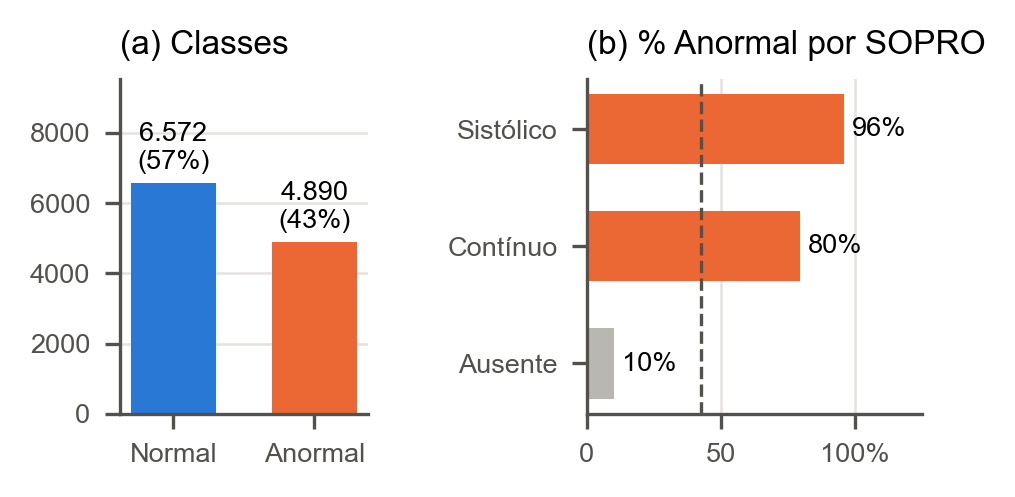
\includegraphics[width=\columnwidth]{fig1_eda.png}
\caption{(a) Distribuição do alvo após a limpeza. (b) Percentual de Anormal por tipo de sopro; a linha tracejada é a taxa global. A separação quase perfeita evidencia o vazamento.}
\label{fig:eda}
\end{figure}

\section{Metodologia}
\textbf{Pré-processamento.} A limpeza (A1) foi aplicada antes da divisão porque usa apenas regras de domínio e não depende do alvo. Ela padroniza grafias, recalcula a IDADE a partir das datas, trata valores impossíveis como ausentes, recalcula o IMC e recalcula a PPA pelas tabelas pediátricas de pressão arterial~\cite{nhbpep2004}. Também foram excluídos, além do SOPRO: ID e convênio (sem relação com o diagnóstico), as datas (usadas só para a idade), HDA~2 e PAS/PAD (mais de 50\% ausentes; a informação fica na PPA) e o IMC (atributo derivado de Peso e Altura). Restaram 11 atributos. Todas as transformações dependentes dos dados ficam dentro de um \textit{pipeline} e são ajustadas somente nos dados de treino de cada dobra:
\begin{itemize}
\item numéricos (IDADE, Peso, Altura, FC): imputação pela mediana com indicador de ausência, log1p em Peso e FC (assimetria positiva) e padronização \textit{z-score};
\item PPA: codificação ordinal (Normal $<$ Pré-hipertensão $<$ HAS~1 $<$ HAS~2) com indicadores de pressão não aferida ou não calculável;
\item nominais (SEXO, B2, PULSOS, HDA~1, MOTIVO1, MOTIVO2): categoria ``Desconhecido'' para ausentes e \textit{one-hot}, agrupando categorias com menos de 20 casos;
\item alvo: Normal~=~0, Anormal~=~1.
\end{itemize}

\textbf{Validação.} Divisão \textit{holdout} estratificada em treino (\Ntreino{} objetos, 80\%) e teste (\Nteste{}, 20\%). Os hiperparâmetros foram escolhidos por busca em grade com validação cruzada estratificada de 5 dobras, apenas no treino. O teste foi usado uma única vez por modelo. A semente é fixa (42) em todas as etapas.

\textbf{Métricas.} A ROC-AUC orienta a escolha do modelo, por não depender do limiar. Também são relatadas a acurácia balanceada, a precisão, a sensibilidade (\textit{recall}) e o F1 da classe Anormal. A sensibilidade recebe atenção especial, porque um falso negativo é uma cardiopatia não encaminhada.

\textbf{Algoritmos} (scikit-learn~\cite{pedregosa2011}). (i)~\textit{Dummy}, que prevê sempre a classe majoritária, como referência mínima. (ii)~Regressão Logística, o baseline simples e interpretável (grade: $C$ e \textit{class\_weight}). (iii)~Random Forest~\cite{breiman2001} com 300 árvores (profundidade, mínimo de amostras por folha e \textit{class\_weight}). (iv)~HistGradientBoosting~\cite{friedman2001,ke2017}, \textit{boosting} de árvores (taxa de aprendizado, profundidade e número de iterações).

\section{Resultados e Discussão}
\textbf{Comparação.} A Tabela~\ref{tab:modelos} resume os resultados. Os três modelos superam com folga a referência \textit{Dummy}, cuja acurácia de \DummyAcc{} com sensibilidade zero mostra por que a acurácia sozinha engana. Os modelos de árvore superam levemente a Regressão Logística na validação, mas as diferenças (menos de 0,01 de AUC) são menores que o desvio entre as dobras. Na prática, os três desempenham de forma equivalente. O Random Forest (\RFparams) teve a maior AUC na validação (\MelhorAUCcv{}~$\pm$~\MelhorAUCcvdp) e foi escolhido. No teste obteve AUC \MelhorAUC{}, acurácia balanceada \MelhorBAcc{}, precisão \MelhorPrec{} e sensibilidade \MelhorRec{}. A proximidade entre validação e teste indica que não houve sobreajuste à seleção de hiperparâmetros.

\begin{table}[!t]
\caption{Comparação dos modelos: ROC-AUC na validação cruzada (média $\pm$ desvio, 5 dobras) e métricas no conjunto de teste (classe positiva = Anormal, limiar 0,5)}
\label{tab:modelos}
\centering
\footnotesize
\setlength{\tabcolsep}{3pt}
\begin{tabular}{@{}lcccccc@{}}
\toprule
 & AUC (CV) & AUC & Ac. bal. & Prec. & Sens. & F1 \\
\midrule
\TabModelos
\bottomrule
\end{tabular}
\end{table}

\textbf{Análise dos erros.} A matriz de confusão (Fig.~\ref{fig:roc}b) mostra \FN{} falsos negativos entre \Nanormalteste{} pacientes Anormais e \FP{} falsos positivos. Os erros não se distribuem igualmente: a sensibilidade é de \RecMenorUm{} em menores de 1 ano, cai para \RecUmTres{} entre 1 e 3 anos e para \RecSeteOnze{} entre 7 e 11, e chega a apenas \RecAdol{} entre 11 e 19 anos. As cardiopatias de lactentes, em geral congênitas e com sinais mais evidentes, são reconhecidas; já as dos adolescentes (arritmias e doenças adquiridas) não se distinguem bem com os atributos disponíveis.

\begin{figure}[!t]
\centering
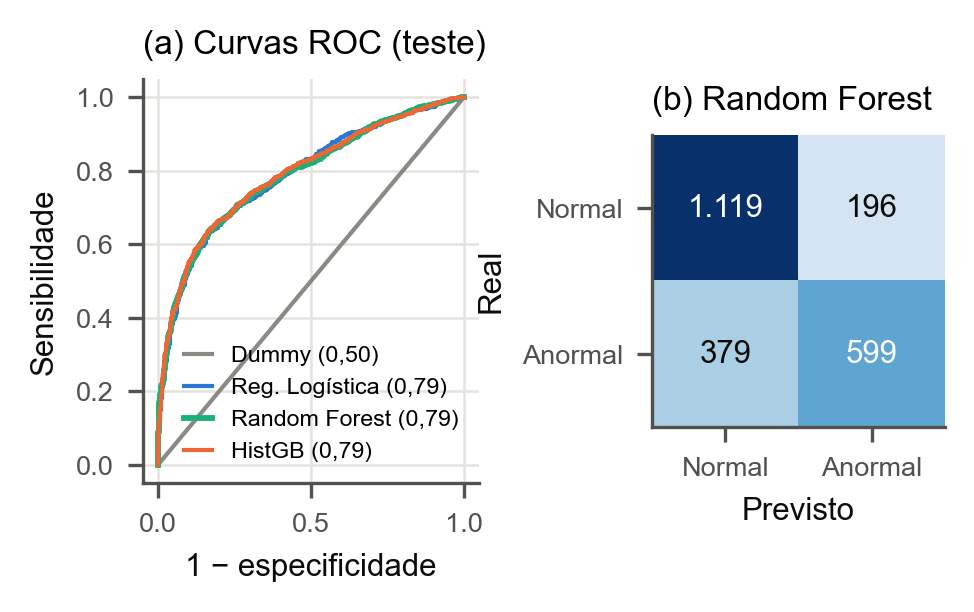
\includegraphics[width=\columnwidth]{fig2_roc_matriz.png}
\caption{(a) Curvas ROC no teste (AUC na legenda). (b) Matriz de confusão do Random Forest no teste, com limiar 0,5.}
\label{fig:roc}
\end{figure}

\textbf{Limiar de decisão.} Para triagem, deixar de encaminhar um doente custa mais que um encaminhamento desnecessário. Escolhemos então um novo limiar sobre as previsões fora da dobra no treino, o menor que atinge sensibilidade de 0,80 ali, e o aplicamos ao teste. Com limiar \Limiar{}, a sensibilidade no teste sobe de \MelhorRec{} para \LimRec{}: os falsos negativos caem de \FN{} para \LimFN{}. Em troca, a precisão cai para \LimPrec{} (\LimFP{} falsos positivos). A AUC não muda, pois só o ponto de operação foi deslocado.

\textbf{Importância dos atributos.} A importância por permutação no teste (Fig.~\ref{fig:imp}) aponta MOTIVO2 (queda de AUC de \ImpMotivoDois), MOTIVO1 (\ImpMotivoUm), B2 (\ImpBdois), FC (\ImpFC) e HDA~1 (\ImpHDA) como os atributos mais relevantes. Peso, Altura e IDADE contribuem pouco isoladamente, porque são fortemente correlacionados entre si e um substitui o outro na permutação. Os coeficientes da Regressão Logística concordam e dão a direção do efeito. B2 hiperfonética (+\CoefBhiper), pulsos femorais diminuídos (+\CoefPulsos) e encaminhamento por ``sopro'' (+\CoefMotSopro) aumentam a chance de Anormal, enquanto B2 normal a reduz (\CoefBnormal). Isso é coerente com o guia diagnóstico do material da disciplina.

\begin{figure}[!t]
\centering
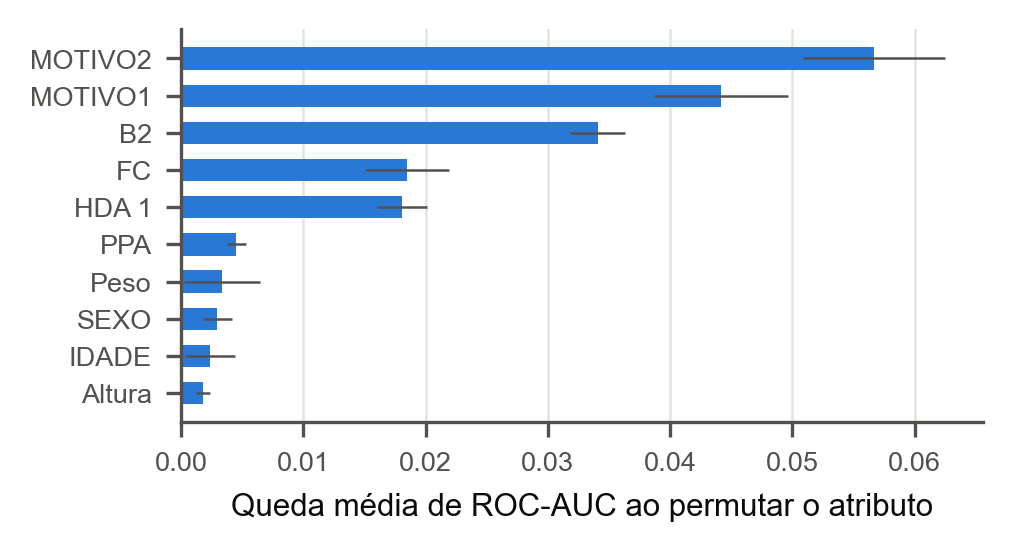
\includegraphics[width=\columnwidth]{fig3_importancia.png}
\caption{Importância por permutação (Random Forest, teste): queda média de ROC-AUC ao embaralhar cada atributo, com o desvio de 10 repetições.}
\label{fig:imp}
\end{figure}

\textbf{Sensibilidade a atributos suspeitos.} A Tabela~\ref{tab:sens} repete a validação cruzada do Random Forest em três configurações. Com o SOPRO, o desempenho seria artificialmente alto, como discutido na Seção~II. No outro extremo, sem MOTIVO1 e MOTIVO2 a AUC cai para \SensSemMotAUC{} e a sensibilidade para \SensSemMotRec{}. O motivo do encaminhamento carrega a suspeita do médico que encaminhou: a categoria ``sopro'' do MOTIVO2 é uma forma indireta do atributo excluído, e ``cardiopatia já estabelecida'' indica diagnóstico prévio. Esses dados existem antes da consulta e foram mantidos. Ainda assim, parte do desempenho vem do julgamento clínico anterior, e não dos sinais objetivos do paciente.

\begin{table}[!t]
\caption{Random Forest na validação cruzada (treino) com diferentes conjuntos de atributos}
\label{tab:sens}
\centering
\footnotesize
\begin{tabular}{@{}lccc@{}}
\toprule
Configuração & AUC & Ac. bal. & Sens. \\
\midrule
Modelo final (sem SOPRO) & \SensFinalAUC & \SensFinalBAcc & \SensFinalRec \\
Com SOPRO (vazamento) & \SensSoproAUC & \SensSoproBAcc & \SensSoproRec \\
Sem SOPRO e sem MOTIVO1/2 & \SensSemMotAUC & \SensSemMotBAcc & \SensSemMotRec \\
\bottomrule
\end{tabular}
\end{table}

\section{Conclusão}
O pré-processamento cuidadoso e a exclusão do SOPRO resultaram em modelos honestos, com ROC-AUC próxima de 0,79 no teste. Random Forest e HistGradientBoosting empataram na prática com a Regressão Logística, o que favorece o modelo linear quando a interpretabilidade importa. Para uso em triagem, o ajuste do limiar eleva a sensibilidade a \LimRec{} ao custo de mais encaminhamentos.

As principais limitações são: (i)~a sensibilidade baixa em adolescentes; (ii)~a dependência do motivo do encaminhamento, que reflete uma avaliação clínica prévia; (iii)~a PPA recalculada com o percentil 50 de estatura, pois a base não traz o percentil individual; e (iv)~os dados virem de um único hospital, o que limita a generalização. Como trabalhos futuros, sugerimos modelos específicos por faixa etária, aprendizado sensível a custos (pesos maiores para falsos negativos), a avaliação em dados de outros centros e o uso do texto livre do histórico clínico.

\section*{Uso de Inteligência Artificial}
O assistente Claude (Anthropic), via Claude Code, apoiou a escrita do código Python (limpeza, modelagem e gráficos) e a redação preliminar deste texto. Todas as decisões, resultados e o texto final foram revisados pelo grupo.

\begin{thebibliography}{9}
\bibitem{fayyad1996} U. Fayyad, G. Piatetsky-Shapiro e P. Smyth, ``From data mining to knowledge discovery in databases,'' \emph{AI Magazine}, vol. 17, n. 3, pp. 37--54, 1996.
\bibitem{nhbpep2004} National High Blood Pressure Education Program Working Group, ``The fourth report on the diagnosis, evaluation, and treatment of high blood pressure in children and adolescents,'' \emph{Pediatrics}, vol. 114, n. 2, pp. 555--576, 2004.
\bibitem{pedregosa2011} F. Pedregosa \emph{et al.}, ``Scikit-learn: Machine learning in Python,'' \emph{J. Mach. Learn. Res.}, vol. 12, pp. 2825--2830, 2011.
\bibitem{breiman2001} L. Breiman, ``Random forests,'' \emph{Machine Learning}, vol. 45, n. 1, pp. 5--32, 2001.
\bibitem{friedman2001} J. H. Friedman, ``Greedy function approximation: a gradient boosting machine,'' \emph{Ann. Statist.}, vol. 29, n. 5, pp. 1189--1232, 2001.
\bibitem{ke2017} G. Ke \emph{et al.}, ``LightGBM: A highly efficient gradient boosting decision tree,'' in \emph{Adv. Neural Inf. Process. Syst. (NeurIPS)}, 2017, pp. 3146--3154.
\bibitem{pinto2004} V. C. Pinto Jr. \emph{et al.}, ``Situação das cirurgias cardíacas congênitas no Brasil,'' \emph{Rev. Bras. Cir. Cardiovasc.}, vol. 19, n. 2, 2004.
\end{thebibliography}

\end{document}
